%%%%%%%%%%%%Outline%%%%%%%%%%%%%%%%%%

%%%
% message<opening: the tight ISA coupling and simple JIT from §2 have a measurable performance cost>
% connect to Background §2.2: eBPF has tightest verification-ISA coupling and no cross-instruction optimization
% this section shows the combination has a real performance cost
% §3.1 quantifies the performance gap, §3.2 traces the underlying ISA cause, §3.3 surveys existing approaches and their limits, §3.4 states the design insight

%%% Section 3.1 The Performance Gap

%%%
% message<methodology: 54 benchmarks in 7 categories, compiled through two pipelines>
% 54 pure-computation micro benchmarks in 7 categories (ALU/bitops, memory, control flow, dep chains, loops, program scale, code cloning)
% (1) LLVM directly: C to native code (upper bound)
% (2) LLVM eBPF backend + eBPF JIT compiler: C to eBPF bytecode, then to native
% both pipelines use the same LLVM compiler front-end and optimization passes

%%%
% message<result: eBPF JIT compiler is 3.0× slower overall, 2.1×–4.7× across categories>
% eBPF JIT compiler is 3.0× slower than native on average
% figure shows geomean of execution time per category
% gap varies: large programs 4.7×, dep chains 4.0×, loops 2.1×
% largest per-benchmark slowdowns in rotates, endian loads, conditional selects
% next section examines these missing operations

%%% Section 3.2 Case Study: 64-bit Rotate

%%%
% message<rotate slowdown comes from missing eBPF opcode, not from the JIT>
% concrete example: 64-bit rotate-left, compiled through both pipelines (figure)
% LLVM x86-64 backend: recognizes rotate idiom, emits single ROL
% LLVM eBPF backend: no rotate opcode in eBPF ISA
% backend decomposes into eight eBPF instructions
% eBPF JIT compiler translates 1:1 to native instructions
% two pipelines share source, compiler, target hardware
% bottleneck: missing rotate opcode in eBPF ISA
% per-instruction encoding cannot supply a missing opcode

%%%
% message<rotate is not isolated — five classes of hardware instructions have no eBPF opcode>
% rotate not an isolated case
% table lists five classes without eBPF opcodes
% eBPF JIT compiler emits multi-instruction sequence for what hardware does in one or two instructions

%%% Section 3.3 Why Existing Approaches Cannot Close This Gap

%%%
% message<bytecode-level optimization cannot reach this gap>
% prior optimizers (K2, Merlin, EPSO) optimize bytecode before loading
% these tools improve the bytecode the eBPF verifier sees
% no bytecode optimization can supply opcodes the eBPF ISA lacks

%%%
% message<in-kernel optimization invalidates the formal verification proofs>
% in-kernel optimization could be cross-instruction JIT or new verifier passes
% either approach invalidates proofs built on the current architecture
% Jitterbug proves per-opcode correctness in isolation
% proof breaks once JIT transforms across instruction boundaries

%%%
% message<extending the eBPF ISA with new opcodes is impractical>
% extending eBPF ISA is also impractical
% each new opcode requires verifier + arch-specific JITs + LLVM + upstream review
% cost scales as O(opcodes × architectures), since different platforms need different instructions

%%% Section 3.4 Insight

%%%
% message<verification and execution need different representations>
% verification needs simple, architecture-independent bytecode the verifier already understands
% execution needs richer representation mapping to hardware-specific instructions
% current design forces both roles onto one ISA; this is the root of the performance gap

%%%
% message<to decouple these two roles, we introduce \lang>
% \lang is extended eBPF bytecode with separate representations for verification and execution
% §4 describes the design in detail

%%%%%%%%%%%%Outline%%%%%%%%%%%%%%%%%%

% zhengjie: motivation experiments are run on VM, not bare metal
% zhengjie: llvmbpf is slower than kernel JIT, 8.1x, probably bacause due to per call overhead in QEMU VM

\section{Motivation}
\label{sec:motivation}

The previous section showed that eBPF couples its ISA to the verifier more tightly than any comparable bytecode system, while the eBPF JIT compiler performs no cross-instruction optimization. This section shows that the combination has a measurable performance cost.
%
\S\ref{subsec:gap} quantifies the performance gap, \S\ref{subsec:rootcause} traces the underlying ISA cause, \S\ref{subsec:approaches} surveys existing approaches and their limits, and \S\ref{subsec:insight} states the design insight.

\subsection{The Performance Gap in Kernel JIT}
\label{subsec:gap}

To quantify the performance cost of the eBPF JIT compiler, we compile 54 pure-computation eBPF micro benchmarks through two pipelines and compare the results. Each program is compiled (1)~directly from C to native code using LLVM (\texttt{clang} \texttt{-O2}), and (2)~from C to eBPF bytecode using the LLVM eBPF backend, then to native code via the eBPF JIT compiler. Both pipelines use the same LLVM front-end and the same middle-end optimization passes; the only difference is the compilation target.

The eBPF JIT compiler is 3.0$\times$ slower than native on average. Figure~\ref{fig:perf-gap} shows the geometric mean of execution time per category. The gap varies across categories: large programs (4.7$\times$) and dependency chains (4.0$\times$) suffer the most, while loops (2.1$\times$) suffer the least. Within each category, the largest slowdowns appear in benchmarks that exercise hardware operations absent from the eBPF ISA, such as rotates (5.8$\times$), endian-aware loads (up to 6.6$\times$), and conditional selects (up to 4.1$\times$). The next section examines these missing operations in detail.

\begin{figure}[t]
\centering
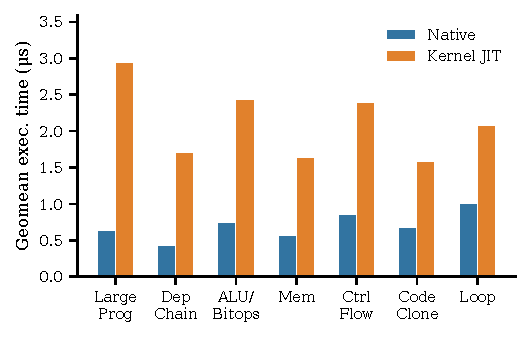
\includegraphics[width=\columnwidth]{figures/sec-3-perf-gap.pdf}
\caption{Geometric mean of execution time per benchmark category for the eBPF JIT compiler relative to native code (LLVM \texttt{-O2}). The 54 benchmarks span seven categories: ALU/bit operations, memory access, control flow, dependency chains, loops, program scale, and code cloning.}
\label{fig:perf-gap}
\end{figure}

\subsection{Case Study: 64-bit Rotate}
\label{subsec:rootcause}

To understand where the slowdown comes from, we examine a concrete example: a 64-bit rotate-left operation, compiled through both pipelines (Figure~\ref{fig:jit-dump}). The LLVM x86-64 backend recognizes the rotate idiom and emits a single \texttt{ROL} instruction. The LLVM eBPF backend, targeting the same source, cannot emit a rotate because the eBPF ISA has no such opcode. The backend decomposes the operation into eight eBPF instructions. The eBPF JIT compiler then translates these eight eBPF instructions one by one to eight x86-64 instructions. The two pipelines share the source code, the LLVM compiler, and the target hardware. The bottleneck is the missing rotate opcode in the eBPF ISA. The eBPF JIT compiler's per-instruction encoding optimizations (\S\ref{subsec:ebpf}) cannot supply a missing opcode.

\begin{figure}[t]
  \centering
  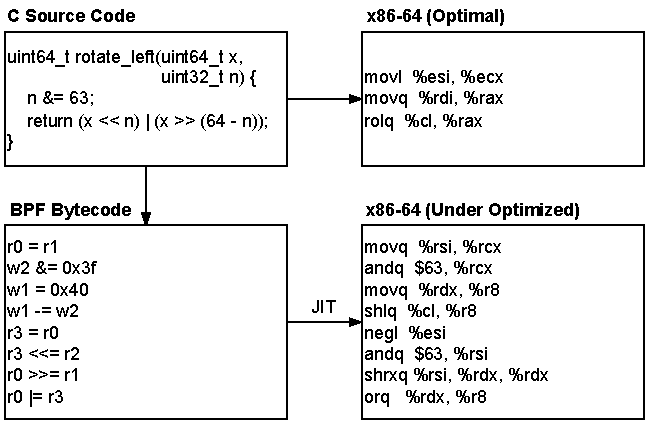
\includegraphics[width=\linewidth]{figures/sec-3-jit-dump.pdf}
  \caption{Compiling a 64-bit rotate through two paths. The direct path compiles C to x86-64 with LLVM, emitting a single \texttt{ROL}. The eBPF path compiles C to eBPF bytecode and then to x86-64 via the eBPF JIT compiler, emitting a longer sequence because the eBPF ISA has no rotate opcode.}
  \label{fig:jit-dump}
\end{figure}


The rotate is not an isolated case. Table~\ref{tab:isa-gap} lists five classes of hardware instructions that have no eBPF opcode equivalent. In each case, the eBPF JIT compiler must emit a multi-instruction sequence for an operation that the hardware performs in one or two instructions.

\input{tables/sec-3-isa-gap}

\subsection{Limitations of Existing Approaches}
\label{subsec:approaches}

Prior work has attempted to close this gap by optimizing eBPF bytecode before loading~\cite{xu2021synthesizing,mao2024merlin,zhu2025epso}. These tools improve the bytecode that the eBPF verifier sees. No bytecode optimization can supply opcodes that the eBPF ISA lacks, such as rotate, conditional move, and wide load.

In-kernel optimization could add logic to either the eBPF JIT compiler (such as cross-instruction transforms) or the verifier pipeline (such as new analysis passes). Either change would invalidate the formal verification proofs built around the current architecture (\S\ref{subsec:formal}). Jitterbug~\cite{nelson2020specification} proves that each opcode is translated correctly in isolation. The proof does not hold once the eBPF JIT compiler transforms programs across instruction boundaries.

Extending the eBPF ISA with new opcodes is also impractical. Each new opcode requires a verifier transfer function, code-generation rules in every architecture-specific JIT backend, updates to the LLVM backend, and upstream kernel review. Since different platforms need different instructions (x86 \texttt{ROL} vs.\ ARM64 \texttt{ROR}), the cost scales as $O(\text{opcodes} \times \text{architectures})$.

\subsection{Decoupling Verification from Execution}
\label{subsec:insight}

Our insight is that verification and execution make conflicting demands on the bytecode. Verification needs a simple, architecture-independent representation that the verifier already understands. Execution needs a richer representation that maps to hardware-specific instructions the eBPF JIT compiler can emit directly. The current eBPF design forces both roles onto a single ISA, causing the performance gap.

To decouple these two roles, we introduce \lang, an extended eBPF bytecode that uses separate representations for verification and execution. \S\ref{sec:design} describes the design.
